\documentclass[12pt]{article}

% Language setting
% Replace `english' with e.g. `pathspanish' to change the document language
\usepackage[english]{babel}

% Set page size and margins
% Replace `letterpaper' with`a4paper' for UK/EU standard size
\usepackage[a4paper,top=2cm,bottom=2cm,left=3cm,right=3cm,marginparwidth=1.75cm]{geometry}

% Useful packages
\usepackage{amsmath}
\usepackage{graphicx}
\usepackage[colorlinks=true, allcolors=black]{hyperref}


%title
\title{\underline{AutoPylot}}
\date{}

\author{%
    \\
    Maxime Ellerbach \\
    Mickael Bobovitch \\
    Alexandre Girold \\
    Maxime Gay \\ \\
    Group: Autonomobile 
    }

\begin{document}
\maketitle
\newpage

\tableofcontents
\newpage

\section{Introduction}

\subsection{Project nature}
Autonomous cars will likely dominate our roads in a relatively close future,
with this project, we aim to have a first approach to such a complex problem.
We will be using a 1:10 scale radio controlled car transformed into a small autonomous car !

\subsection{State of the art}

In this section, we will try to see what was previously made in this sector of industry.
It would not be realistic to compare our 1:10 project to real sized cars such as Tesla's, simply because in a racing environnement,
we don't need to deal with such an amount of safety: pedestrian detection, emergency braking, speed limit detection and other.
So we will only see miniature autonomous racing framework that we would likely race against.\\

The most known is called "DonkeyCar", created by Will Roscoe and Adam Conway in early of 2017. Most of the models trained with DonkeyCar are behavior cloning models, meaning models that tries to replicate the behavior of a driver. This methods uses a big amount of images (input) associated to steering angles and throttle (output), it requires the user to drive the car (collect data) prior to training the model: no examples means no training. The lack of training data often leads to the car leaving the track.\\

One other framework worth looking at is one created by Nvidia called "JetRacer" released in 2019. It uses a different approach from DonkeyCar where the user annotates the images by hand by clicking on where the car should go. The model used is similar to what DonkeyCar uses meaning a Convolutional Neural Network with one input (the image) and two outputs, one for the steering angle and one for the throttle to apply.

\section{Objectives}

\subsection{Final objectives}
Our main objective is to make our car race against other cars and win the race !
This will require multiple intermediate milestones:
\begin{itemize}
\item Being able to send scripted controls to the motor and servo
\item Being able to drive the car manually using a controller
\item Develop a way to gather images and annotations and store them in a stuctured way, for example sorted by date
\item Process those data before feeding them to the neural network
\item Being able to train a convolutional neural network using those data
\item Tweak the architecture and the parameters of the chosen model to acheive the best results
\item 
\end{itemize}

\subsection{Optional objectives}
Those are the opt objectives

\subsection{Motivations}
Those are the final requirements

\section{Technical specifications}

\subsection{Hardware}
Those are the technical specifications
- what we need
- what will we use ?

\rotatebox[origin=c]{-90}{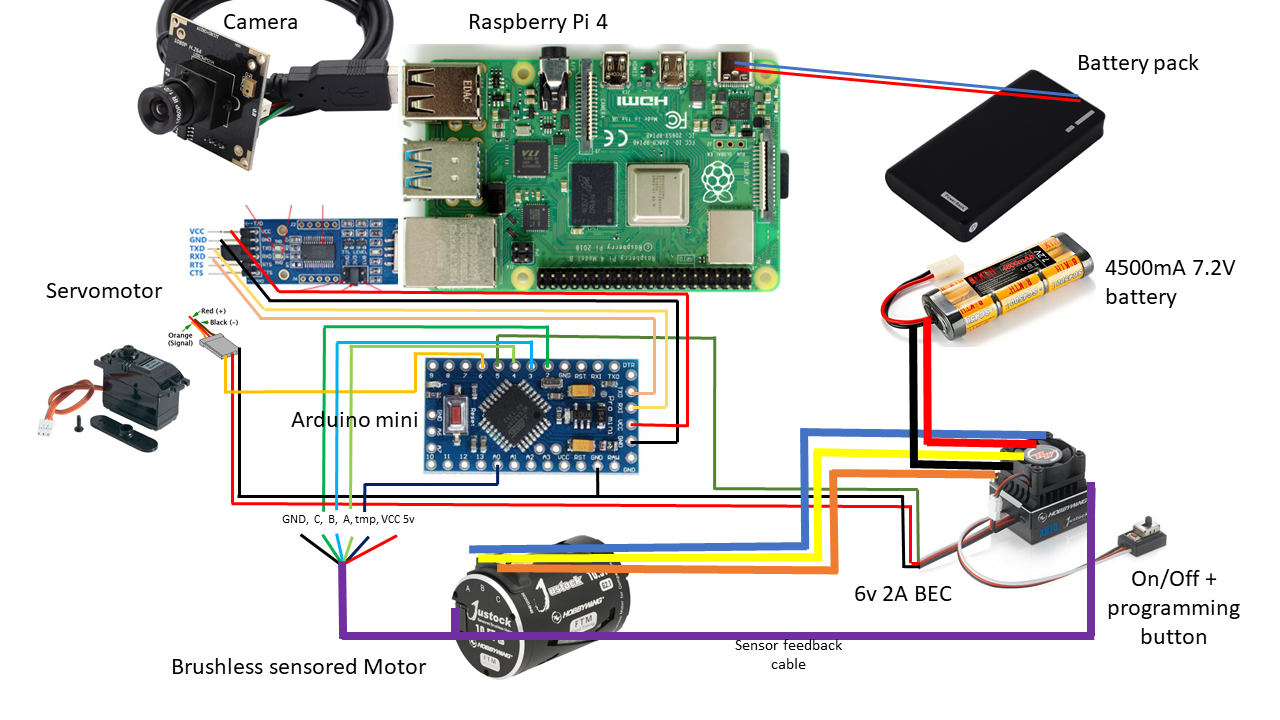
\includegraphics[width=27cm]{schema.png}}

\subsection{Software}
- data generation / gathering
- what software parts we will need

\subsection{Constraints}
- weight
- language: python
- autonomous navigation
- data ?
- framerate, efficiency of the algorithm
- safety

\section {Planning}

\section {Task allocation}

\section {Conclusion}



\end{document}